\documentclass[twoside,10pt]{article}
\usepackage{amsmath,amsfonts,amsthm,fullpage,amssymb}
%\usepackage{mymath}
\usepackage{algorithm,amsmath,amssymb}
\usepackage{algorithmic}
\usepackage{graphicx, color}
\usepackage{url}


\begin{document}


\title{ISYE 6740 Homework 5 \\ 
Fall 2024\\ 
Prof. Yao Xie\\
 Total 100 points}
\date{}
\maketitle



%As usual, please submit a report with sufficient explanation of your answers to each the questions, together with your code, in a zip folder.

%----------------------------------------------------------------------------------

%feature selection (CV, bias-variance tradeoff), Boosting, random forest 



\subsection*{1. Comparing multi-class classifiers for handwritten digits classification. (20 points)}

This question is to compare different classifiers and their performance for multi-class classifications on the complete MNIST dataset at \url{http://yann.lecun.com/exdb/mnist/}. You can find the data file \textbf{mnist\_10digits.mat} in the homework folder. The MNIST database of handwritten digits has a training set of 60,000 examples and a test set of 10,000 examples. We will compare {\bf KNN, logistic regression, SVM, kernel SVM, and neural networks}. 

\begin{itemize}

\item We suggest you to ``standardize'' the features before training the classifiers by dividing the values of the features by 255 (thus mapping the range of the features from [0, 255] to [0, 1]).

\item You may adjust the number of neighbors $K$ used in KNN to have a reasonable result (you may use cross-validation but it is not required; any reasonable tuning to get a good result is acceptable). Only the best k needs to be reported.

\item You may use a neural networks function \textsf{sklearn.neural\_network} with \textsf{hidden\_layer\_sizes = (20, 10)}. 


\item For kernel SVM, you may use radial basis function kernel and choose the proper kernel.

\item For KNN and SVM, you can randomly downsample the training data to size $m=5000$, to improve the computation efficiency. 

\item Packages may be used for all models in this problem
\end{itemize}

Train the classifiers on the training dataset and evaluate them on the test dataset.

\begin{enumerate}

	\item (15 points) Report confusion matrix, precision, recall, and F-1 score for each of the classifiers. For the precision, recall, and F-1 score of each classifier, we will need to report these for each of the digits. So you can create a table for this. For this question, each of the 5 classifiers, {\bf KNN, logistic regression, SVM, kernel SVM, and neural networks}, accounts for 3 points.
	\item (5 points) Comment on the performance of the classifier and give your explanation why some of them perform better than others.	
\end{enumerate}


\subsection*{2. SVM (25 points).}

\begin{enumerate}
\item (5 points) Explain why can we set the margin $c = 1$ to derive the SVM formulation? Justify using a mathematical proof.
\item (5 points) Using Lagrangian dual formulation, show that the weight vector can be represented as
\[
w = \sum_{i=1}^n \alpha_i y_i x_i.
\]
where $\alpha_i \geq 0$ are the dual variables. What does this imply in terms of how to relate data to $w$?
\item (5 points) Explain why only the data points on the ``margin'' will contribute to the sum above, i.e., playing a role in defining $w$. Hint: use the Lagrangian multiplier derivation and KKT condition we discussed in class. 

\item Simple SVM by hand. 

Suppose we only have four training examples in two dimensions as shown in Fig. The positive samples at $x_1 = (0, 0)$, $x_2 = (2, 2)$ and negative samples at $x_3 = (h, 1)$ and $x_4 = (0, 3)$. 
%
\begin{center}
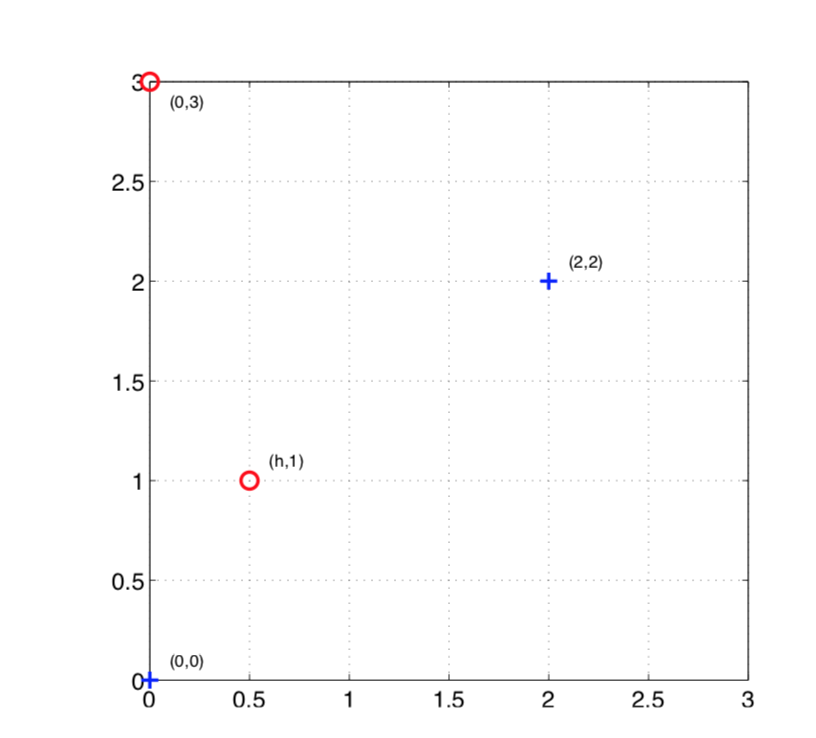
\includegraphics[width = 0.5\textwidth]{svm}
\end{center}

\begin{enumerate}
\item (5 points) For what range of parameter $h > 0$, the training points are still linearly separable?



\item (5 points) Does the orientation of the maximum margin decision boundary change as $h$ changes, when the points are separable? Please explain your conclusion.
\end{enumerate}


\end{enumerate}


\subsection*{3. Neural networks and backpropagation. (15 points)}


Consider a simple two-layer network in the lecture slides. Given $m$ training data $(x^i, y^i)$, $i = 1, \ldots, m$, the cost function used to training the neural networks
\[
\ell(w, \alpha, \beta) = \sum_{i=1}^m (y^i - \sigma(w^T z^i))^2
\]
where $\sigma (x) = 1/(1+e^{-x})$ is the sigmoid function, $z^i$ is a two-dimensional vector such that  $z_1^i = \sigma(\alpha^T x^i)$, and $z_2^i = \sigma(\beta^T x^i)$.
\\
Be sure to show all steps of your proofs.

\begin{enumerate}
\item (5 points) Show that the gradient is given by
\[
\frac{\partial \ell(w, \alpha, \beta) }{\partial w}
= - \sum_{i=1}^m 2(y^i - \sigma(u^i))\sigma(u^i)(1-\sigma(u^i)) z^i,
\]
where $u^i = w^T z^i$. 
\item (10 points) Also, show the gradient of $\ell(w, \alpha, \beta)$ with respect to $\alpha$ and $\beta$ and write down their expression.
\end{enumerate}


\subsection*{4. Feature selection and change-point detection. (20 points)} 

\begin{enumerate}

\item (10 points) Consider the mutual information-based feature selection. Suppose we have the following table (the entries in the table indicate counts) for the spam versus and non-spam emails:
%
\begin{center}
\begin{tabular}{c|c|c}
\hline
& ``prize'' = 1 & ``prize'' = 0 \\\hline
``spam'' = 1 & 150& 10 \\ \hline 
 ``spam'' = 0 & 1000 & 15000  \\\hline
\end{tabular}
\end{center}

\begin{center}
\begin{tabular}{c|c|c}
\hline
& ``hello'' = 1 & ``hello'' = 0 \\\hline
``spam'' = 1 & 145 & 15 \\ \hline 
 ``spam'' = 0 & 11000 & 5000  \\\hline
\end{tabular}
\end{center}

Given the two tables above, calculate the mutual information for the two keywords, ``prize`` and ``hello'' respectively. Which keyword is more informative for deciding whether or not the email is spam? If any tools are used for your calculation, you must still show your mathematical steps in your report and include code/files used for your calculations.

\item  (10 points)  Given two distributions, $f_0 = \mathcal{N}(0, 1)$, $f_1 = \mathcal{N}(0, 1.5)$, derive what should be the CUSUM statistic (i.e., show the mathematical CUSUM detection statistic specific to these distributions). Plot the CUSUM statistic for a sequence of 150 randomly generated i.i.d. (independent and identically distributed) samples, $x_1, \ldots, x_{100}$ according to $f_0$ and $x_{101}, \ldots, x_{150}$ according to $f_1$. Please provide a reasonable estimation based solely on your plot of where a change may be detected.


\end{enumerate}


\subsection*{5. Medical imaging reconstruction (20 points).} 

In this problem, you will consider an example resembles medical imaging reconstruction in MRI.  We begin with a true image image of dimension 50 $\times$ 50 (i.e., there are 2500 pixels in total). Data is \textsf{cs.mat}; you can plot it first. This image is truly sparse, in the sense that 2084 of its pixels have a value of 0, while 416 pixels have a value of 1. You can think of this image as a toy version of an MRI image that we are interested in collecting.

Because of the nature of the machine that collects the MRI image, it takes a long time to measure each pixel value individually, but it's faster to measure a linear combination of pixel values. We measure $n$ = 1300 linear combinations, with the weights in the linear combination being random, in fact, independently distributed as $\mathcal{N}(0,1)$. Because the machine is not perfect, we don't get to observe this directly, but we observe a noisy version. These measurements are given by the entries of the vector
\[
y = A x + \epsilon,
\]
where $y \in \mathbb R^{1300}$, $A \in \mathbb R^{1300\times 2500}$, and $\epsilon \sim \mathcal N(0, 25\times I_{1300})$ where $I_n$ denotes the identity matrix of size $n\times n$. In this homework, you can generate the data $y$ using this model. 

Now the question is: can we model $y$ as a linear combination of the columns of $x$ to recover some coefficient vector that is close to the image? Roughly speaking, the answer is yes. 

Key points here: although the number of measurements $n$ = 1300 is smaller than the dimension $p$ = 2500, the true image is sparse. Thus we can recover the sparse image using few measurements exploiting its structure. This is the idea behind the field of \textit{compressed sensing}. 

The image recovery can be done using lasso
\[
\min_x \|y-Ax\|_2^2 + \lambda \|x\|_1.
\]
\begin{enumerate}
\item (10 points) Now use lasso to recover the image and select $\lambda$ using 10-fold cross-validation. Plot the cross-validation error curves, and show the recovered image using your selected lambda values.

\item (10 points) To compare, also use ridge regression to recover the image:
\[
\min_x \|y-Ax\|_2^2 + \lambda \|x\|_2^2.
\]
Select $\lambda$ using 10-fold cross-validation. Plot the cross-validation error curves, and show the recovered image using your selected lambda values. Which approach gives a better recovered image?
\end{enumerate}



\end{document}
